\documentclass[a4paper,12pt]{report}
\usepackage{color}
\usepackage{caption}
\usepackage{amsmath}
\usepackage[table,xcdraw]{xcolor}
\usepackage{amssymb}
\usepackage{graphicx}
\usepackage{epstopdf}
\usepackage{listings}
\definecolor{anti-flashwhite}{rgb}{0.95, 0.95, 0.96}
\lstset { %
    language=C++,
    backgroundcolor=\color{lightgray}, % set backgroundcolor
    basicstyle=\small,% basic font setting
}
\begin{document}
\title{
Algorithms: CS2443\\
\begin{large}
Assignment 1
\end{large}
}
\author{Sagar Jain - CS17BTECH11034\\}
\maketitle
\section*{Solutions}
%\subsection*{Points To Note}
\begin{enumerate}
\item The given question can be solved elegantly using the concept of Hamiltonian Paths. \textit{A Hamiltonian Path in a graph is one which visits every vertex exactly once.}
\\Construction of graph from data available:
\begin{enumerate}
\item Label the n players 1-n arbitrarily.
\item We use a directed graph since we have a winner and a loser.
\item Players represent nodes.
\item $\exists$ an edge from node i to node j \textbf{iff} player i won against player j.
\end{enumerate}
Now we know that if there exists an edge from any node i to j, implies player i has won against player j. If we can find an Hamiltonian Path in the graph, then all we have to do is rename the players with their number in the hamiltonian path. This will work since every pair of adjacent vertices in the path have an edge between them i.e. second player of the pair lost to first.
\subsubsection*{The Algorithm}
\textbf{Aim}: To construct a Hammiltonian Path.\\\\
\textbf{Steps}:
\begin{enumerate}
\item Let the node 1 be the first node in the Hamiltonina Path.
\item Loop through every other node (y) to find its position in the Path. We can have three possible cases:
\begin{enumerate}
\item Player y has won against the first player in the path. Insert y at the beginning of the path.
\item Player y has lost to the last player in thepath. Insert y at the end of the path.
\item There exists a k such that player was has lost to the kth player in the path and won against the (k+1)th player in the path. Insert y between the kth and (k+1)th player.
\end{enumerate}
It can be shown that we will always land in one of these three cases. The proof is the same as showing existence of a Hamiltonian Path in a tournament graph.
\end{enumerate}
\subsubsection*{Code}
\begin{lstlisting}
#include<iostream>
#include<assert.h>
#include<vector>

using namespace std;

// Function for checking existence of edge

bool didWin(vector<vector<int>> graph, int a, int b) {
  int i, s = graph[a].size();
  for(i = 0;i < s;i++) {
    if(graph[a][i] == b)
      return true;
  }
  return false;
}

int main()
{
  int n, i, temp1, temp2, j;
  cin >> n;
  vector<vector<int>> graph(n);

// Creating the graph
// Arbitrarily call the players 1 - n  
  for(i = 0;i < n*(n-1)/2;i++) {
    cin >> temp1 >> temp2;
    graph[temp1 - 1].push_back(temp2 - 1);
  }

  vector<int> hamiltonian_path;
  hamiltonian_path.push_back(0);
  for(i = 1;i < n;i++)
  {
    if(didWin(graph ,i,hamiltonian_path.front()))
      hamiltonian_path.insert(
      hamiltonian_path.begin(), i);
    else if(didWin(graph, hamiltonian_path.back(), i))
      hamiltonian_path.push_back(i);
    else {
      for(j=0;j<hamiltonian_path.size();j++) {
        if(didWin(graph,j,i) && didWin(graph,i,j+1)) {
          hamiltonian_path.insert(
          hamiltonian_path.begin()+j+1,i);
          break;
        }
      }
    }
  }
  for(i = 0;i < n;i++) {
    cout<<hamiltonian_path[i]+1 << " ";
  }
  cout << endl;
  
// rename the players in the order of 
// occurence in the path
}
\end{lstlisting}
\subsubsection*{Correctness}
To prove the correctness we need to show that the final list printed satisfies the condition that given any pair of adjacent players in the path, the first player won against the second.\\
This can be achieved by showing the loop invariant holds, the invariant being that at any time in the path given any pair of adjacent players in the path, the first player won against the second.\\
Initially we start with just one node, so the invariant holds true vacuosuly.
Now we show that in any of the three cases of the loop the invariant holds.
\begin{enumerate}
\item Case 1, we add the player y at the beginning of the list only if it has defeated the first player in the path. Since y can exist in only one pair i.e. the first two in the path and the condition holds for this pair, we are done.
\item Case 2, we add y to the end of the list only if it has lost to the last player of the path, Since y can only exist on one pair, i.e. the last two in the path and the condition holds for this pair, we are done.
\item Case 3, we insert y only between kth and (k+1)th if it has, both lost to k and won against k+1, since y can only exist in these two pairs ((k,y),(y, k+1)) and the condition holds for these two pairs, we are done.
\end{enumerate}
\subsubsection*{Complexity}
The computation part of the algorithm is in the two loops, in the worst case, where we have to traverse the entire hamiltonian path for every node, the inner loop would run $n*(n-1)/2$ times.
This gives us a comlexity of $O(n^2)$.
\item The given question can be solved using an approach similar to binary search for sorted arrays.\\
The problem in the question is the fact that the array can be circularly shifted. If not for this, the answer would always be min(first element, last element).\\
To overcome this problem we can consider the entire sequence to be circular i.e. no specific last or first element.The way we do this is by defining the element at index i as $arr_{i\:mod\:n}$.
In the algorithm the idea is to descend down a trough till we find an element less than both of its adjacent elements i.e. the minimum no. of the array.\\
Note: A trough is any triplet in the array such that $i<j<k$ and $arr_i>arr_j<arr_k$
\subsubsection*{The Algorithm}
\textbf{Aim}:To find the minimum of the bitonic array.\\\\
\textbf{Steps/Pseudo Code}:\\
\begin{enumerate}
\item We start by comparing $arr_0$ and $arr_{n/2}$, if $arr_0 > arr_{n/2}$ then the first trough is 0, n/2 and n (n mod n = 0) else the first trough is n/2, n, 3*n/2 (3*n/2 mod n = n/2).
\item Now, we repeatedly decrease the size of this trough to end up at the minimum. Call the trough a,b,c.
\item If $|a-b|>|b-c|$ then we work in between a,b else between b,c. WLG assume the inequality holds. We then get the value of $arr_{(a+b)/2}$. If $arr_{(a+b)/2} > arr_b$ then the new trough is (a+b)/2, b, c else the new trough is a, (a+b)/2, b.
\item On every iteration we check if the middle element is infact the minima(by comparing with both the adjacent elements) and when we find it we break out of the loop.
\end{enumerate}
\textbf{Example Run}
Take the array [2,-2, 10, 13, 21, 18, 6]
First we take the middle element $arr_{7/2 = 3} = 13 > arr_0 = 2 \implies$ the first trough is 3, 7, 10.\\
$ \because |7-3| > |10-7|$ next element checked is $arr_{(7+3)/2 = 5} = 18$\\
$\because 18>arr_7$ our new trough is 5, 7, 10.
$ \because |10-7| > |5-7|$ next element checked is $arr_{(10+7)/2 = 8} = -2$\\
Clearly -2 is less than both its adjacent elements (i.e. 2,10) and as it is a bitonic array this has to be unique, $\therefore min(arr) = -2$
\subsubsection*{Correctness}
Points to note for correctness:
\begin{enumerate}
\item The minimum value of the array has to be in the trough. Since there is only one minima.
\item We reduce the size of our array always keeping the trough in it.
\end{enumerate}
(a) and (b) $\implies$ that we are converging to the minimum, as we check at every iteration if we have found the required element, it will be found at or before we are left with a one element array.
\subsubsection*{Complexity}
At every iteration we reduce the size of our array. The possible reductions in array size our, n/4 when the mid of one side of trough is greater than previous mid, or n/2 when it is less (since we started by making our first trough at half length of array, this pattern will follow thorughout, this is not necessary and other ways could make the convergence faster). So the array either becomes 3/4th of initial or half of initial every iteration.
It is clear to see that at most after $log_{4/3}n$ iterations we will be left with an array of size one.
$\therefore$ the complexity of this algorithm is $O(logn)$.
\item \begin{enumerate}
\item $T (n) <= 2T (5n/7) + n log n $\\\\
Using master theorem,\\
\begin{align*}
a &= 2\\
b &= 7/5\\
log_ba &> 2\\
f(n) &= nlogn\\
\end{align*}
We know that, $\exists$ $c \leqslant 2$ st $n^c = O(f(n)) = O(nlogn) \implies c < log_ba\\\implies T(n) = O(n^{log_ba}) = O(n^{log_{7/5}2})\;(\approx n^{2.06}) $
\item \begin{align*}
f(n) &\leqslant f(4n/5) + f(n/6) + n\\
&\leqslant f(4n/5) + f(n/5) + n\\
&\leqslant f(16n/25) + f(n/25) + f(4n/25) + f(4n/25) + 2n\\
...\\
&\leqslant kn\\
k &= log_{5/4}n = O(logn)\\
\implies f(n) &= O(nlogn)
\end{align*}
\item
\begin{align*}
g(n) &= \sum_{k=1}^{n} {klogk}\\
g'(n) &= \int_{1}^{n} xlogx dx
\end{align*}
We can approximate g(n) with $g'(n)$ to find the upper bound.
\begin{figure}
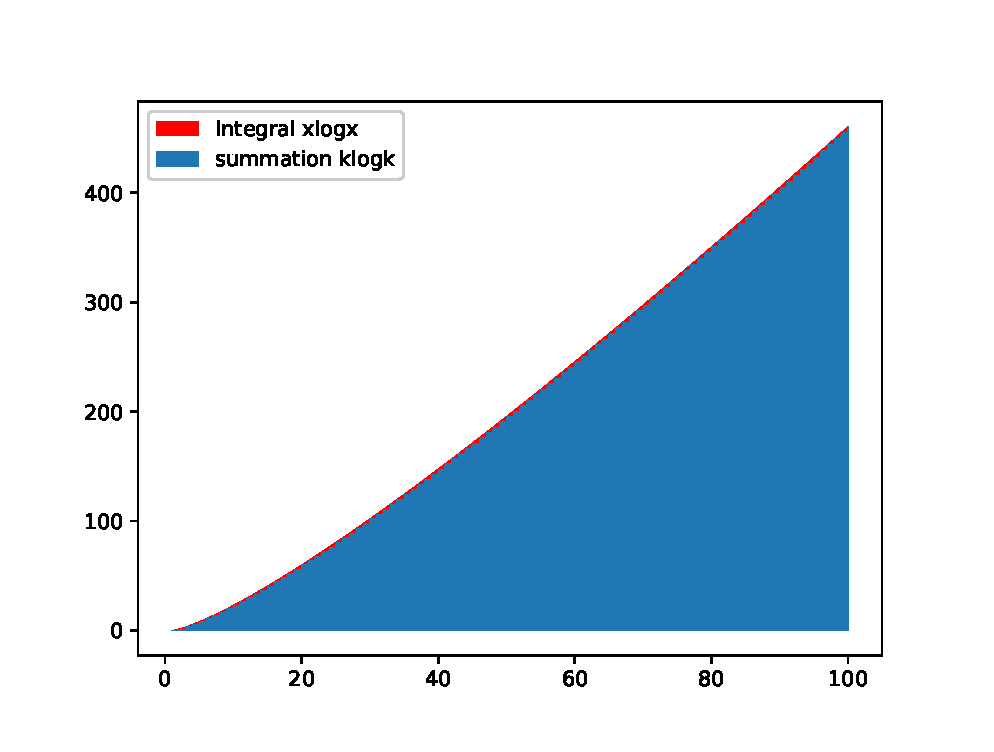
\includegraphics[scale=0.8]{large.eps}
\caption*{Comparision of integraton and summation of xlogx}~\\\\
As visible, for large n, the difference between the two is negligible. So, we can use the approximation to get the upper bound.
\begin{align*}
g(n) &\leqslant g'(n)\\
g'(n) &= \int_{1}^{n} xlogx dx\\
&= logx*x^2/2 - x^2/4 \Big|_1^n\\
&= O(n^2logn)\\
&\therefore g(n) =  O(n^2logn)
\end{align*}
\end{figure}
\end{enumerate}
\end{enumerate}
\end{document}